\newpage
\newsection{User Management}
\subsection{Aggregates}
\subsubsection{User}
\begin{itemize}
	\item \textbf{UserId}: this attribute must be unique and refers to the \emph{user\_id} key in the corresponding \emph{Auth0} users table(without first 6 characters 'Auth0|' );
	\item \textbf{FirstName}: user's first name;
	\item \textbf{LastName}: user's  last name;
	\item \textbf{Date}: user's birth date;
	\item \textbf{Email}: this attribute must be unique and respect the right format;
	\item External links:
	\begin{itemize}
		\item \textbf{Role}: user's role;
		\item \textbf{Group}: user's belonging group.
	\end{itemize}
\end{itemize}

\subsubsection{Role}
\begin{itemize}
	\item \textbf{RoleId}: is a UUID;
	\item \textbf{Name}: this attribute must be unique;
	\item \textbf{Desc}: role's description;
	\item External links:
	\begin{itemize}
		\item \textbf{Auth}: JSON array of role's authorizations.
	\end{itemize}
\end{itemize}

\subsubsection{Authorization}
\begin{itemize}
	\item \textbf{AuthId}: is a UUID;
	\item \textbf{Name}: this attribute must be unique;
	\item \textbf{Desc}: auth's description.
\end{itemize}

\subsubsection{Group}
\begin{itemize}
	\item \textbf{GroupId}: is a UUID;
	\item \textbf{Name}: this attribute must be unique;
	\item \textbf{Desc}: group's description.
\end{itemize}

\subsection{Admin side}
\subsubsection{Authentication}
The authentication feature is provided by a third-party provider, Auth0. In the admin side only administrators can log in; the client must be signed into the corresponding application's database on Auth0.
\subsubsection{Use cases}

\begin{figure}[H]
	\centering
	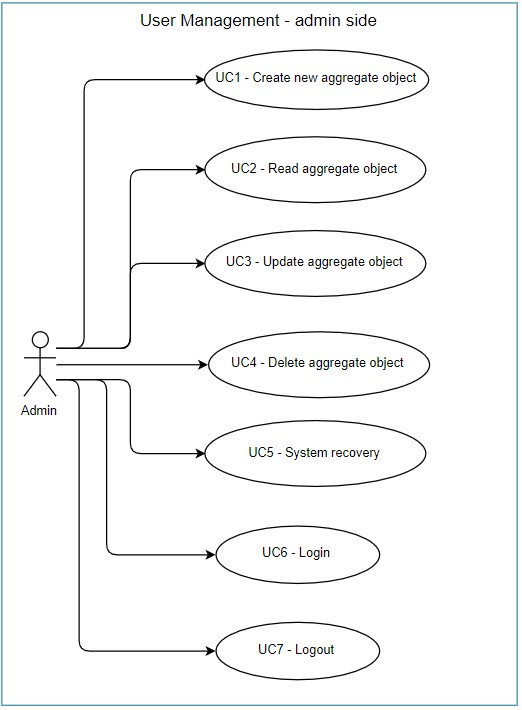
\includegraphics[scale=1.2]{../Img/UC_admin}
	\caption{Admin use cases}\label{}
\end{figure}

\begin{itemize}
	\item UC1: the admin creates a new object based on the type of aggregate;
	\item UC2: the admin reads the information about an object based on the type of aggregate;
	\item UC3: the admin updates an object based on the type of aggregate;
	\item UC4: the admin deletes an object;
	\item UC5: the admin recovers the system state from the chosen timestamp re-running of the event occurred after that; 
	\item UC6: the admin logs in into the application using the Auth0 portal;
	\item UC7: the admin logs out from the application.
\end{itemize}
	

\subsection{User side}
\subsubsection{Authentication}
The authentication feature is provided by a third-party provider, Auth0. In the user side only users can log in; he can sign in with email and password or using Google's authentication or just logs in using his credentials.
\subsubsection{Use cases}

\begin{figure} [H]
	\centering
	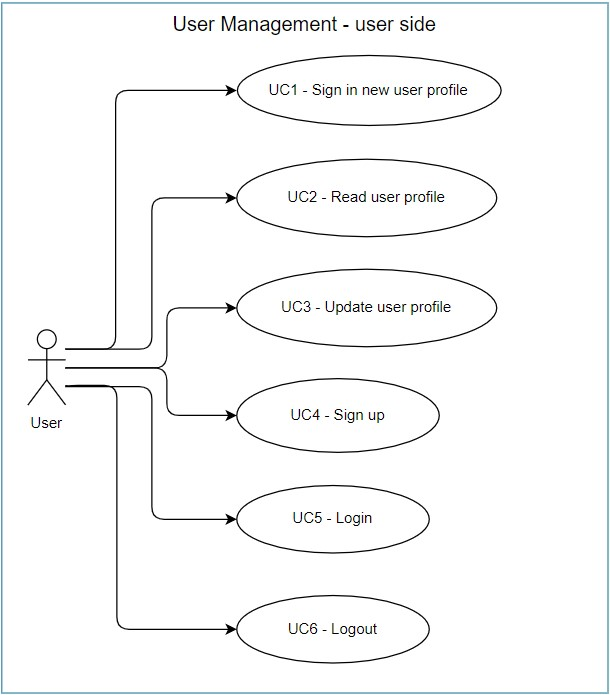
\includegraphics[scale=1.2]{../Img/UC_user}
	\caption{User use cases}\label{}
\end{figure}

\begin{itemize}
	\item UC1: the user fills the form to sign in into the application the first time logs in;
	\item UC2: the user reads his profile;
	\item UC3: the user updates his profile;
	\item UC4: the user signs up to Auth0 authentication portal using email and password or Google's account;
	\item UC5: the user logs in to Auth0 authentication portal using email and password or Google's account;
	\item UC6: the user logs out from the application.
\end{itemize}

